\subsection{Methods}
To find the first marker, the white from the image is selected using HSV color segmentation.
Then contours are found and white blobs of a certain size and compactness is chosen.
Another method was explored and tested in appendix \ref{sec:using_lines}, using the lines in the image, but was dismissed because it did not find the marker in a majority of the test images.
Tests and reasoning for the segmentation can be found in appendix \ref{sec:full_marker1}.
This method can track a single point which is the center of mass of the blobs within the contours.

The second marker was found using HSV color segmentation to seperate into the relevant colors and Hough transform to find circles.
Tests and reasoning for the second detector can be found in appendix \ref{sec:full_marker2}.
This method can either track the four circles or the center between the circles.
Hough Circles does not handle projection well and the center of the Hough circle thus not guaranteed to be in the center of the projected circle.

In figure \ref{fig:circle_detection} is a normal case from the easy and a worst case example from the hard set shown.
As the robot follows the point, it is not expected to be this bad at any situation so the detector is deemed successful.
The detector find the marker in all but two images from the hard data set.

\begin{figure}[h]
 \centering
 \begin{subfigure}{0.49\linewidth}
 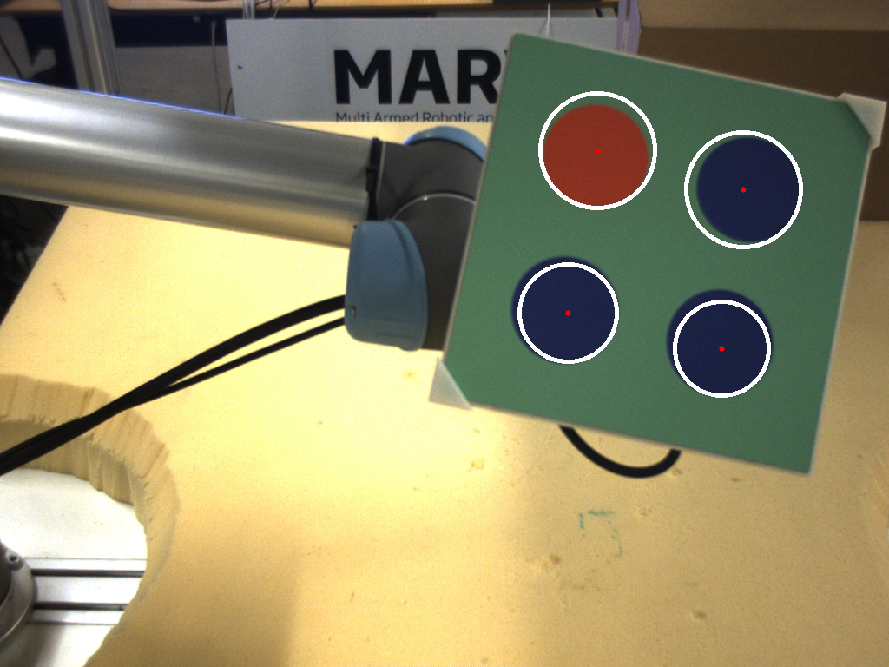
\includegraphics[width=\linewidth]{graphics/best_case_hough_circle}
 \caption{Normal case.}
 \end{subfigure}
 \begin{subfigure}{0.49\linewidth}
 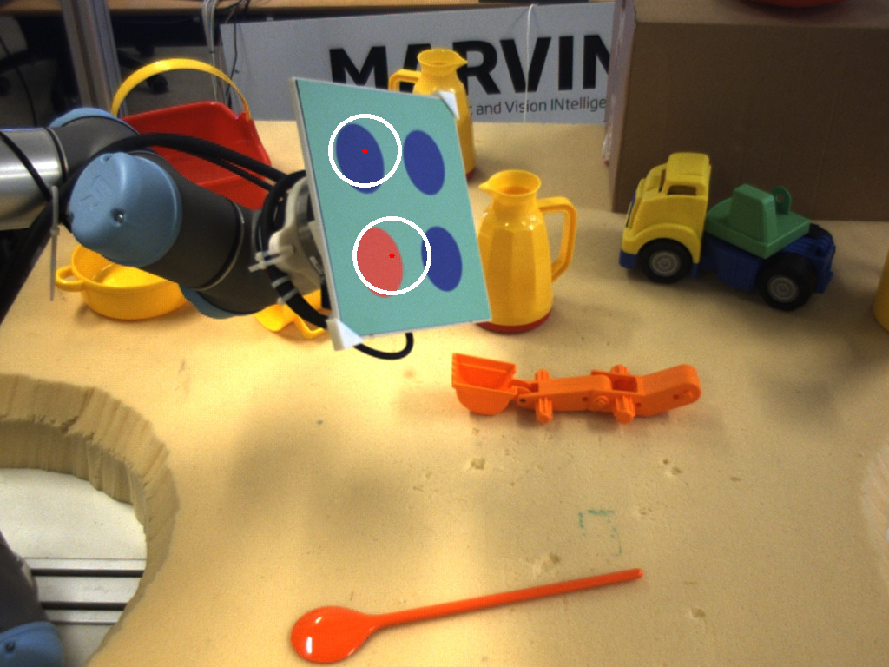
\includegraphics[width=\linewidth]{graphics/worst_case_hough_circle}
 \caption{Worst case.}
 \end{subfigure}
 \caption{Detecting circles with and without projection.}
 \label{fig:circle_detection}
\end{figure}


The third marker was found using SIFT image descriptors.
SIFT was found to be slow, so an optimization was implemented in form of a controller which crops the image around the previously known position of the marker.
This proved to be reliable if the marker did not move too far, which is the situation when a robot follows the point of a marker.
Tests and reasoning for the second detector can be found in appendix \ref{sec:full_marker3}.
The detector can either return the center of the image or the corners of the marker.